% =====================================================================
%  GPU-Accelerated Monte Carlo Simulation for Financial Option Pricing
%  BLG 562E -- Parallel Computing for GPUs using CUDA (Spring 2026, ITU)
%  Authors: Talha Sarlik, Mehmet Bedirhan Onder
%
%  Build:   pdflatex poster.tex   (run twice for cross-references)
%  Layout:  a0 portrait, 3 columns, ITU CEng template flow.
% =====================================================================
\documentclass[portrait,a0b,final]{a0poster}

% ---------- Packages -------------------------------------------------
\usepackage[utf8]{inputenc}
\usepackage[T1]{fontenc}
\usepackage{lmodern}
\usepackage{microtype}
\usepackage[a0paper,margin=22mm]{geometry}

\usepackage{amsmath,amssymb,amsfonts}
\usepackage{graphicx}
\usepackage{booktabs}
\usepackage{array}
\usepackage{xcolor}
\usepackage[most]{tcolorbox}
\usepackage{tikz}
\usetikzlibrary{positioning,arrows.meta,shapes,calc}
\usepackage{listings}
\usepackage{enumitem}
\setlist{nosep,leftmargin=*}

\graphicspath{{figures/}}

% ---------- ITU palette ---------------------------------------------
\definecolor{ituBlue}   {RGB}{0,  60,120}
\definecolor{ituRed}    {RGB}{198, 12, 48}
\definecolor{ituGold}   {RGB}{198,156, 38}
\definecolor{blockBg}   {RGB}{245,248,253}
\definecolor{blockBorder}{RGB}{200,210,225}

% ---------- Block style (custom \posterblock command) ----------------
\newtcolorbox{posterblock}[1]{%
  enhanced,
  colback=blockBg, colframe=blockBorder,
  arc=4mm, boxrule=0.6mm,
  left=8mm, right=8mm, top=4mm, bottom=4mm,
  title={\strut\textbf{\Large #1}},
  fonttitle=\bfseries,
  colbacktitle=ituBlue, coltitle=white,
  attach boxed title to top left={xshift=10mm, yshift=-6mm},
  boxed title style={colframe=ituBlue, arc=2mm, boxrule=0.4mm,
                     left=5mm, right=5mm, top=1.2mm, bottom=1.2mm},
  before skip=8mm, after skip=8mm,
}

% ---------- Body type ------------------------------------------------
\renewcommand{\familydefault}{\sfdefault}     % sans body
\linespread{1.06}

% =====================================================================
\begin{document}
\pagestyle{empty}

% =====================================================================
%  Title banner
% =====================================================================
\begin{tcolorbox}[enhanced, colback=ituBlue, colframe=ituBlue,
                  arc=4mm, boxrule=0pt, left=10mm, right=10mm,
                  top=8mm, bottom=6mm]
\centering
\color{white}
{\Huge\bfseries GPU-Accelerated Monte Carlo Simulation\\
for Financial Option Pricing\par}
\vspace{6mm}
{\LARGE Talha Sarlık (704241052) \quad$\cdot$\quad Mehmet Bedirhan Önder (704251026)\par}
\vspace{3mm}
{\large BLG 562E -- Parallel Computing for GPUs using CUDA \quad$\cdot$\quad
Asst. Prof. Ayşe Yılmazer \quad$\cdot$\quad Spring 2026\par}
{\large Faculty of Computer and Informatics Engineering \quad$\cdot$\quad
Istanbul Technical University\par}
\end{tcolorbox}

\vspace{6mm}

% =====================================================================
%  Three columns
% =====================================================================
\noindent
\begin{minipage}[t]{0.315\textwidth}
% =================== Column 1 ========================================

\begin{posterblock}{Introduction}
Monte Carlo (MC) is the standard tool for pricing path-dependent
financial options when no closed-form solution exists. For European
options the analytical Black--Scholes formula provides exact ground
truth, which we use as a \emph{validation oracle}.
\par\medskip
The algorithm is \textbf{embarrassingly parallel}: each simulated
price path is an independent random walk under Geometric Brownian
Motion. This makes MC a textbook fit for CUDA -- but extracting the
parallelism requires careful attention to memory hierarchy and
reduction patterns.
\end{posterblock}

\begin{posterblock}{Motivation}
A single-threaded CPU prices one European call at $5\times10^{7}$
paths in about \textbf{1.6\,s}. The same workload on a consumer
GTX~1650 takes \textbf{$\sim$1\,ms}. Translating this textbook
parallelism into $>$1000$\times$ wall-clock speedup is not automatic
-- the difference between a naive and an optimised kernel is itself a
\textbf{3.7$\times$ kernel-level speedup}, and an unsafe FP32 atomic
reduction produces a \emph{numerically wrong} answer at large $N$.
This poster quantifies that gap and identifies the bottleneck per
implementation with Nsight Compute.
\end{posterblock}

\begin{posterblock}{Contributions}
\begin{enumerate}
\item Three progressively-tuned CUDA kernels for European MC option
      pricing: \texttt{mc\_naive} (global atomics), \texttt{mc\_shared}
      (block-level reduction), \texttt{mc\_antithetic} (variance
      reduction).
\item Validation against the analytical Black--Scholes price to
      within sub-$\sigma$ tolerance at $N=10^{6}$.
\item Profiler-driven bottleneck analysis: each optimisation step is
      justified by a specific Nsight Compute signal (atomic
      contention $\rightarrow$ compute-bound).
\item Reproducible benchmark sweep over $10^{4}\!\rightarrow\!5\times10^{7}$
      paths, median of 5 runs.
\item Headline: \textbf{1133$\times$} (shared) and
      \textbf{1652$\times$} (antithetic) speedup over the CPU
      baseline at $N=5\times10^{7}$.
\end{enumerate}
\end{posterblock}

\begin{posterblock}{Algorithm Flow}
% Algorithm flow: GBM sampling -> payoff -> block reduction -> host CI
% Standalone fragment: \input{} this file inside a \block{} on the poster.
\begin{center}
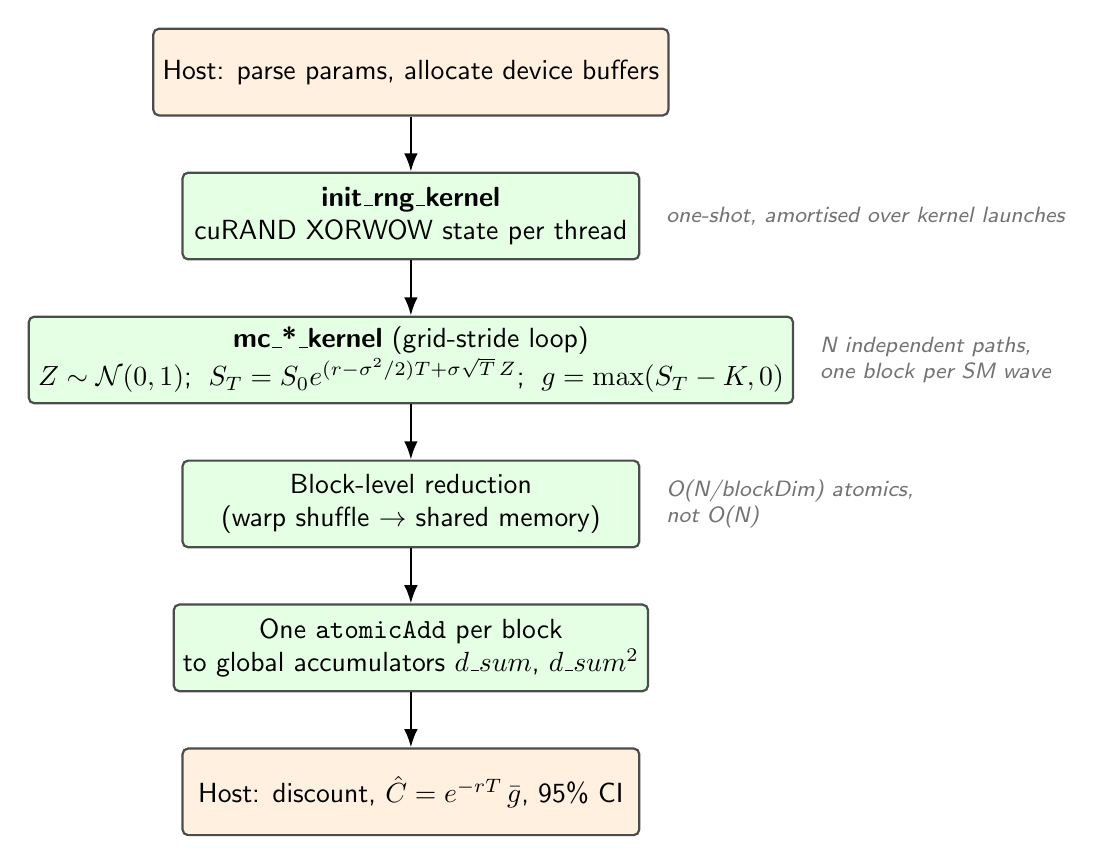
\begin{tikzpicture}[
    >=Latex,
    node distance = 7mm and 10mm,
    box/.style   = {rectangle, rounded corners=2pt, draw=black!70, thick,
                    fill=blue!8, minimum width=58mm, minimum height=11mm,
                    align=center, font=\normalsize},
    gpu/.style   = {box, fill=green!10},
    host/.style  = {box, fill=orange!12},
    note/.style  = {font=\footnotesize\itshape, color=black!55, align=left},
    every path/.style = {thick, ->, >=Latex},
]

\node[host] (init)   {Host: parse params, allocate device buffers};
\node[gpu, below=of init]   (rng)    {{\bfseries init\_rng\_kernel}\\
                                      cuRAND XORWOW state per thread};
\node[gpu, below=of rng]    (loop)   {{\bfseries mc\_*\_kernel} (grid-stride loop)\\
                                      $Z\sim\mathcal{N}(0,1)$;\;
                                      $S_T=S_0e^{(r-\sigma^2/2)T+\sigma\sqrt{T}\,Z}$;\;
                                      $g=\max(S_T-K,0)$};
\node[gpu, below=of loop]   (reduce) {Block-level reduction\\
                                      (warp shuffle $\rightarrow$ shared memory)};
\node[gpu, below=of reduce] (atomic) {One \texttt{atomicAdd} per block\\
                                      to global accumulators $d\_sum$, $d\_sum^2$};
\node[host, below=of atomic] (finish){Host: discount, $\hat{C} = e^{-rT}\,\bar{g}$, 95\% CI};

\draw (init)   -- (rng);
\draw (rng)    -- (loop);
\draw (loop)   -- (reduce);
\draw (reduce) -- (atomic);
\draw (atomic) -- (finish);

\node[note, right=2mm of rng]    {one-shot, amortised over kernel launches};
\node[note, right=2mm of loop]   {N independent paths,\\ one block per SM wave};
\node[note, right=2mm of reduce] {O(N/blockDim) atomics,\\ not O(N)};
\end{tikzpicture}
\end{center}

\end{posterblock}

\end{minipage}%
\hfill
\begin{minipage}[t]{0.315\textwidth}
% =================== Column 2 ========================================

\begin{posterblock}{Problem Definition}
\textbf{European call option.} Right to buy underlying at strike $K$
at expiry $T$. Under Black--Scholes assumptions the underlying
follows Geometric Brownian Motion:
\[
dS_t = r\,S_t\,dt + \sigma\,S_t\,dW_t.
\]
Closed-form for the terminal price (one Euler step is exact under
GBM):
\[
S_T = S_0\exp\!\Bigl(\bigl(r-\tfrac{1}{2}\sigma^{2}\bigr)T
                     + \sigma\sqrt{T}\,Z\Bigr),\quad
Z\sim\mathcal{N}(0,1).
\]
\textbf{Monte Carlo estimator} -- discounted average of $N$ i.i.d.\
payoffs:
\[
\hat{C} = e^{-rT}\,\frac{1}{N}\sum_{i=1}^{N}\max\!\bigl(S_T^{(i)}-K,\,0\bigr).
\]
\textbf{Convergence.} Standard error shrinks as
$\mathcal{O}(N^{-1/2})$: quadrupling $N$ halves the error, motivating
GPU throughput.
\par\smallskip
\textbf{Validation oracle.} Analytical Black--Scholes call
\(
C = S_0\,\Phi(d_1) - K e^{-rT}\Phi(d_2).
\)
\par\smallskip
\textbf{Parameters used throughout:} $S_0=K=100$, $r=0.05$,
$\sigma=0.2$, $T=1.0$. Analytical price $=\mathbf{10.4506}$.
\end{posterblock}

\begin{posterblock}{Kernel Variants}
\textbf{\texttt{mc\_naive}.} One thread per path slice (grid-stride
loop). \texttt{atomicAdd} per path on a global accumulator. Memory
pattern is the bottleneck -- every payoff serialises on
\texttt{*d\_sum}, \emph{and} FP32 accumulation loses precision at
large $N$ (mc\_naive @ $5\!\times\!10^{7}$ paths reports
price~$=9.95$ vs analytical $10.45$).
\par\smallskip
\textbf{\texttt{mc\_shared}.} Each thread accumulates its slice's
$(sum,\,sum^2)$ in \textbf{registers}, then a single
\texttt{block\_reduce\_sum()} (warp shuffle $\rightarrow$ shared-memory
tree $\rightarrow$ thread~0) writes \textbf{one} \texttt{atomicAdd}
per block. Atomic count drops from $\mathcal{O}(N)$ to
$\mathcal{O}(N/\text{blockDim})$.
\par\smallskip
\textbf{\texttt{mc\_antithetic}.} For each $Z$ drawn, evaluate the
payoff at $+Z$ and $-Z$ and average as one effective sample.
Identical block-level reduction as \texttt{mc\_shared}. Halves the
variance for monotonic payoffs (proven for European calls/puts)
without doubling RNG cost.
\par\medskip
\centerline{\textit{Architectural difference, in one figure:}}
\medskip
% Side-by-side schematic of where each kernel performs its reduction.
% \input{} inside a \block{}.
\begin{center}
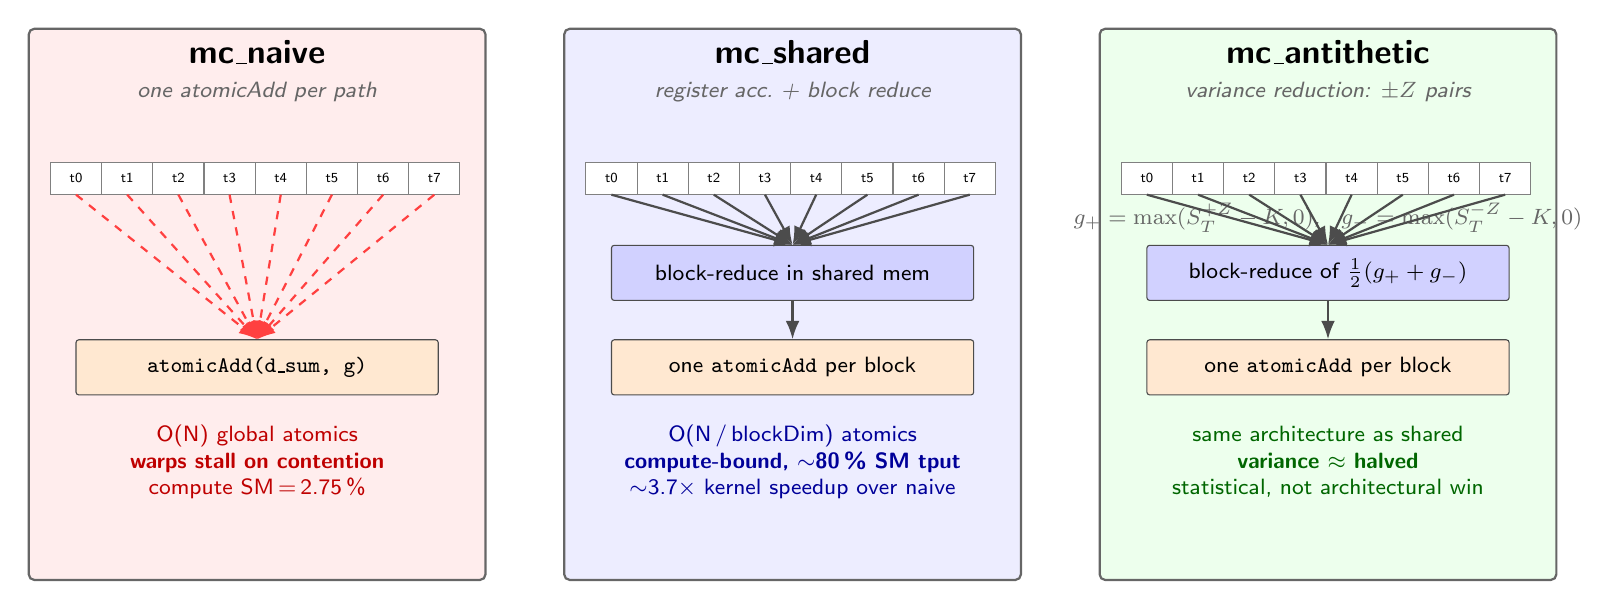
\begin{tikzpicture}[
    >=Latex,
    panel/.style    = {rectangle, rounded corners=2pt, draw=black!60, thick,
                       minimum width=58mm, minimum height=70mm, align=center,
                       inner sep=2mm},
    naive/.style    = {panel, fill=red!7},
    shared/.style   = {panel, fill=blue!7},
    anti/.style     = {panel, fill=green!7},
    head/.style     = {font=\bfseries\large, align=center},
    sub/.style      = {font=\footnotesize\itshape, color=black!60, align=center},
    body/.style     = {font=\footnotesize, align=center},
    thread/.style   = {rectangle, draw=black!50, fill=white, minimum width=6.5mm,
                       minimum height=4mm, inner sep=0pt, font=\tiny},
    glob/.style     = {rectangle, rounded corners=1pt, draw=black!70, fill=orange!18,
                       minimum width=46mm, minimum height=7mm, font=\footnotesize},
    blkacc/.style   = {rectangle, rounded corners=1pt, draw=black!70, fill=blue!18,
                       minimum width=46mm, minimum height=7mm, font=\footnotesize},
    arr/.style      = {->, thick, >=Latex, draw=black!70},
    contend/.style  = {->, thick, >=Latex, draw=red!75, dashed},
]

% =============================== Panel 1: NAIVE ===============================
\begin{scope}[xshift=0mm]
  \node[naive] (P1) at (0, 0) {};
  \node[head]  at (0,  32mm) {\textsc{mc\_naive}};
  \node[sub]   at (0,  27mm) {one atomicAdd per path};
  % 8 threads in a row
  \foreach \i in {0,...,7} {
      \node[thread] (T1_\i) at (-23mm + \i*6.5mm,  16mm) {t\i};
  }
  \node[glob] (G1) at (0, -8mm) {\texttt{atomicAdd(d\_sum, g)}};
  % red dashed arrows showing serialization at the global accumulator
  \foreach \i in {0,...,7} {
      \draw[contend] (T1_\i.south) -- (G1.north);
  }
  \node[body, color=red!75!black] at (0, -20mm)
       {O(N) global atomics\\ \textbf{warps stall on contention}\\
        \footnotesize{compute SM\,$=$\,2.75\,\%}};
\end{scope}

% =============================== Panel 2: SHARED ==============================
\begin{scope}[xshift=68mm]
  \node[shared] (P2) at (0, 0) {};
  \node[head]   at (0,  32mm) {\textsc{mc\_shared}};
  \node[sub]    at (0,  27mm) {register acc.\ + block reduce};
  \foreach \i in {0,...,7} {
      \node[thread] (T2_\i) at (-23mm + \i*6.5mm,  16mm) {t\i};
  }
  \node[blkacc] (B2) at (0,  4mm) {block-reduce in shared mem};
  \node[glob]   (G2) at (0, -8mm) {one \texttt{atomicAdd} per block};
  \foreach \i in {0,...,7} {
      \draw[arr] (T2_\i.south) -- (B2.north);
  }
  \draw[arr] (B2.south) -- (G2.north);
  \node[body, color=blue!60!black] at (0, -20mm)
       {O(N\,/\,blockDim) atomics\\ \textbf{compute-bound, $\sim$80\,\% SM tput}\\
        \footnotesize{$\sim$3.7$\times$ kernel speedup over naive}};
\end{scope}

% =============================== Panel 3: ANTITHETIC ==========================
\begin{scope}[xshift=136mm]
  \node[anti] (P3) at (0, 0) {};
  \node[head] at (0,  32mm) {\textsc{mc\_antithetic}};
  \node[sub]  at (0,  27mm) {variance reduction: $\pm Z$ pairs};
  \foreach \i in {0,...,7} {
      \node[thread] (T3_\i) at (-23mm + \i*6.5mm,  16mm) {t\i};
  }
  % indicate +Z/-Z pairing
  \node[font=\footnotesize\itshape, color=black!60] at (0, 11mm)
       {$g_+ = \max(S_T^{+Z}-K,0)$,\;\; $g_- = \max(S_T^{-Z}-K,0)$};
  \node[blkacc] (B3) at (0,  4mm) {block-reduce of $\tfrac{1}{2}(g_+ + g_-)$};
  \node[glob]   (G3) at (0, -8mm) {one \texttt{atomicAdd} per block};
  \foreach \i in {0,...,7} {
      \draw[arr] (T3_\i.south) -- (B3.north);
  }
  \draw[arr] (B3.south) -- (G3.north);
  \node[body, color=green!40!black] at (0, -20mm)
       {same architecture as shared\\ \textbf{variance $\approx$ halved}\\
        \footnotesize{statistical, not architectural win}};
\end{scope}

\end{tikzpicture}
\end{center}

\end{posterblock}

\begin{posterblock}{Reduction Internals}
% Reduction tree: warp shuffle + shared memory tree -> one atomicAdd.
% \input{} inside a \block{}.
\begin{center}
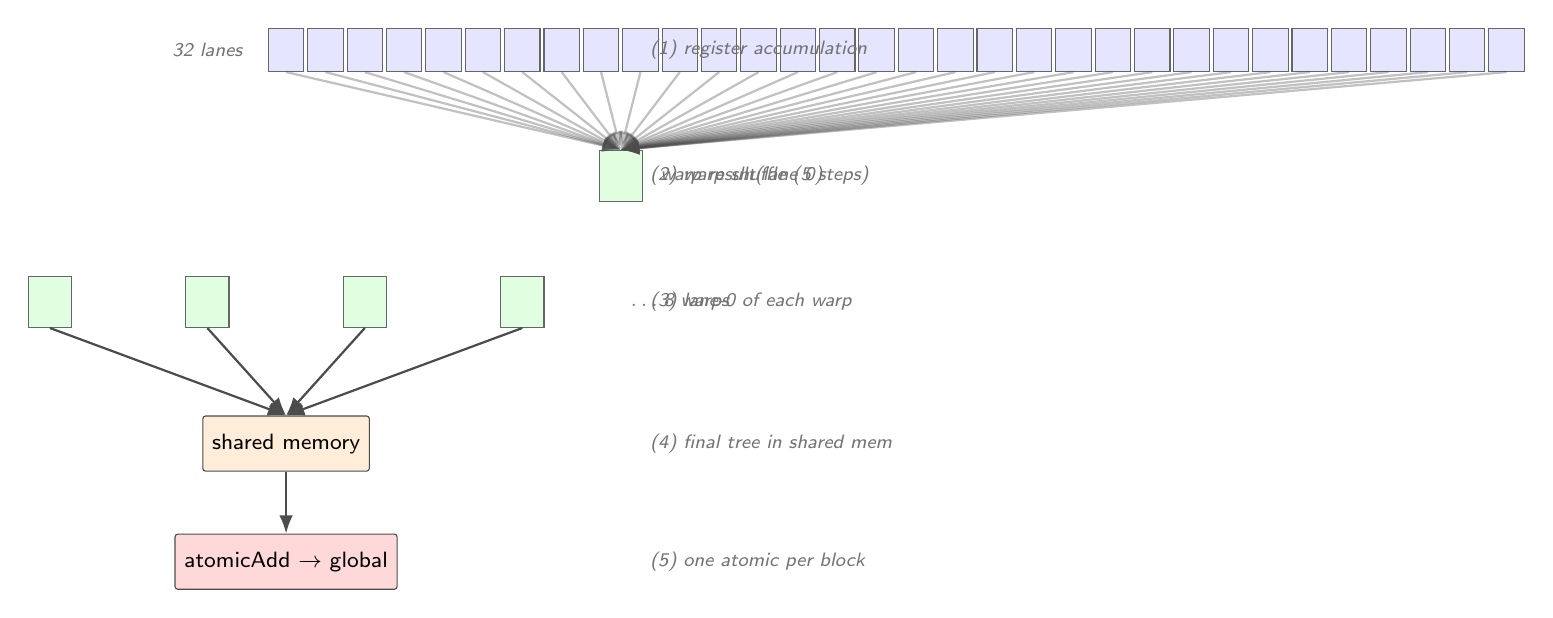
\begin{tikzpicture}[
    >=Latex,
    every node/.style = {font=\footnotesize},
    lane/.style       = {rectangle, draw=black!60, fill=blue!10, minimum width=4.5mm,
                          minimum height=5.5mm, inner sep=0pt},
    warp/.style       = {rectangle, draw=black!60, fill=green!12, minimum width=5.5mm,
                          minimum height=6.5mm, inner sep=0pt},
    blk/.style        = {rectangle, rounded corners=1pt, draw=black!70, fill=orange!15,
                          minimum width=12mm, minimum height=7mm},
    arr/.style        = {->, thick, >=Latex, draw=black!70},
    label/.style      = {font=\scriptsize\itshape, color=black!55},
]

% Row 1: 32 lanes (one warp), per-thread register accumulator
\foreach \i in {0,...,31} {
    \node[lane] (L\i) at (\i*5mm, 0) {};
}
\node[label, left=2mm of L0] {32 lanes};

% Warp-shuffle reduction (5 levels) collapses to lane 0 of the warp.
\node[warp] (W0) at (4*5mm + 9*5mm/2, -16mm) {};
\foreach \i in {0,...,31} {
    \draw[arr, opacity=0.35] (L\i.south) -- (W0.north);
}
\node[label, right=1mm of W0] {warp result\\(lane 0)};

% Imagine 8 warps total (8 in a 256-thread block); show 4 warps for visual clarity.
\node[warp] (W1) at (-30mm, -32mm) {};
\node[warp] (W2) at (-10mm, -32mm) {};
\node[warp] (W3) at ( 10mm, -32mm) {};
\node[warp] (W4) at ( 30mm, -32mm) {};
\node[label] at (50mm, -32mm) {$\ldots$\;8 warps};

\node[blk] (SM) at (0mm, -50mm) {shared memory};
\foreach \w in {W1, W2, W3, W4} {
    \draw[arr] (\w.south) -- (SM.north);
}

% Final reduction in shared memory and one atomicAdd to global.
\node[blk, fill=red!15] (ATOM) at (0mm, -65mm) {atomicAdd $\rightarrow$ global};
\draw[arr] (SM.south) -- (ATOM.north);

% Annotations on the right.
\node[label, anchor=west] at (45mm,   0mm) {(1) register accumulation};
\node[label, anchor=west] at (45mm, -16mm) {(2) warp shuffle (5 steps)};
\node[label, anchor=west] at (45mm, -32mm) {(3) lane-0 of each warp};
\node[label, anchor=west] at (45mm, -50mm) {(4) final tree in shared mem};
\node[label, anchor=west] at (45mm, -65mm) {(5) one atomic per block};

\end{tikzpicture}
\end{center}

\end{posterblock}

\end{minipage}%
\hfill
\begin{minipage}[t]{0.315\textwidth}
% =================== Column 3 ========================================

\begin{posterblock}{Experimental Setup}
\textbf{GPU:} NVIDIA GTX~1650 (\texttt{sm\_75}, 16 SMs, 4\,GB), CUDA
12.4, driver 566.36, Windows~11.\par
\textbf{CPU baseline:} single-threaded, \texttt{-O3 -march=native}.\par
\textbf{Sweep:} $N \in \{10^{4},\,10^{5},\,10^{6},\,10^{7},\,
2.5\!\times\!10^{7},\,5\!\times\!10^{7}\}$.\par
\textbf{Reporting:} median of 5 runs, warmup discarded; warm-cache
kernel time only (does not include the one-shot \texttt{curand\_init}).
\end{posterblock}

\begin{posterblock}{A. Validation}
At $N = 10^{6}$ paths, all four implementations agree with the
analytical Black--Scholes price within 4-$\sigma$:
\par\medskip
\centering
\begin{tabular}{lrrrc}
\toprule
\textbf{Implementation} & \textbf{Estimate} & \textbf{Abs.\ Err.} &
\textbf{$\sigma$} & \textbf{Status}\\
\midrule
\texttt{mc\_cpu}        & 10.4501 & 0.0005 & 0.0 & PASS \\
\texttt{mc\_naive}      & 10.4718 & 0.0212 & 1.4 & PASS \\
\texttt{mc\_shared}     & 10.4719 & 0.0213 & 1.4 & PASS \\
\texttt{mc\_antithetic} & 10.4593 & 0.0088 & 0.8 & PASS \\
\bottomrule
\end{tabular}
\end{posterblock}

\begin{posterblock}{B. Throughput \& Speedup}
\centering
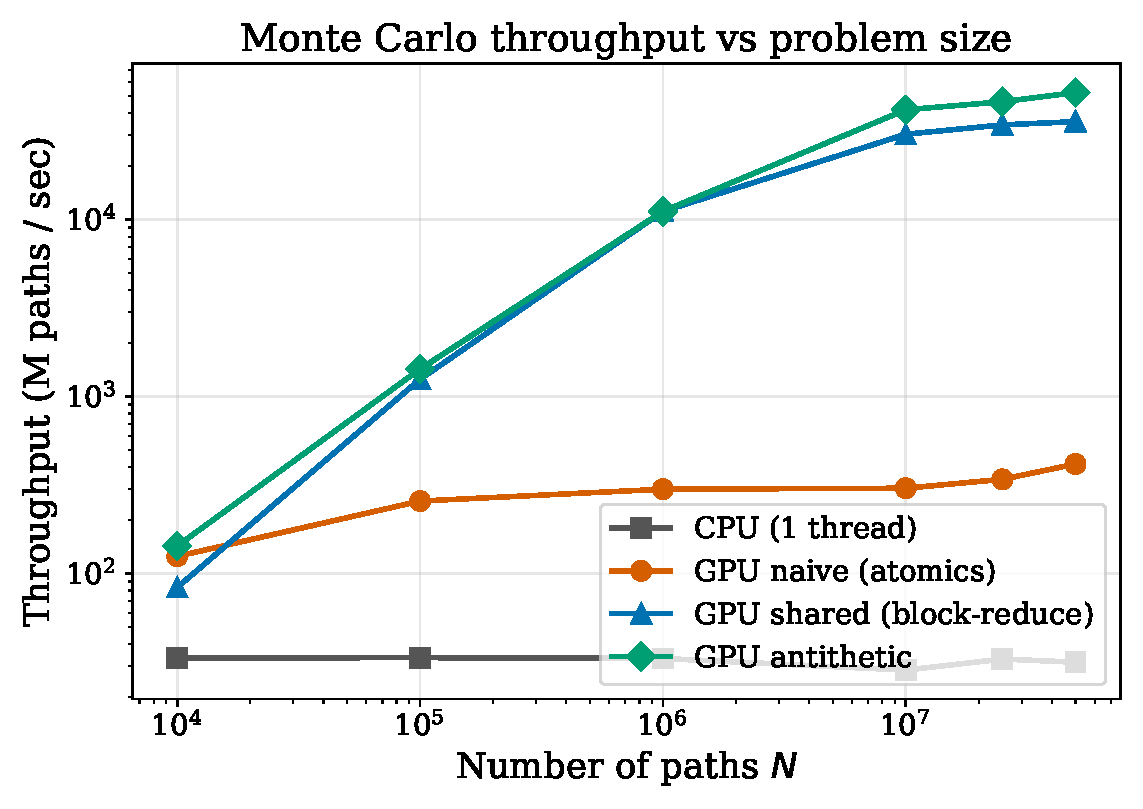
\includegraphics[width=\linewidth]{figures/fig_throughput.pdf}\par
\medskip
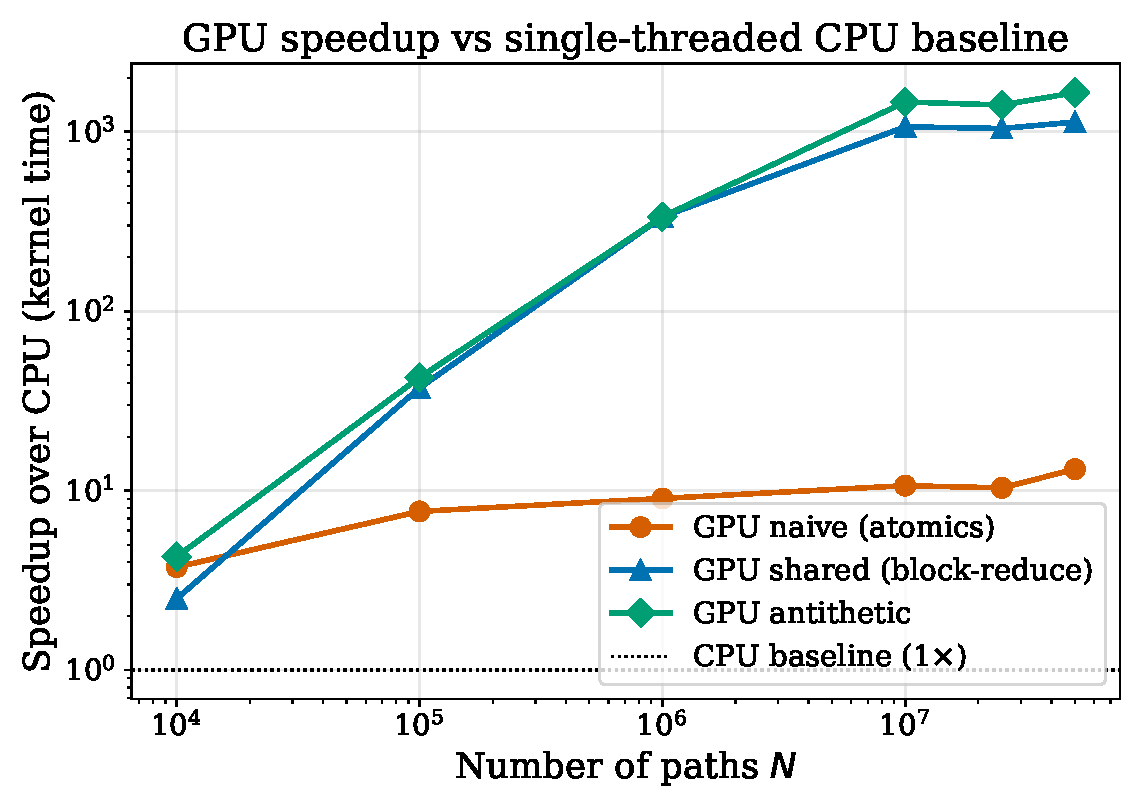
\includegraphics[width=\linewidth]{figures/fig_speedup.pdf}\par
\medskip
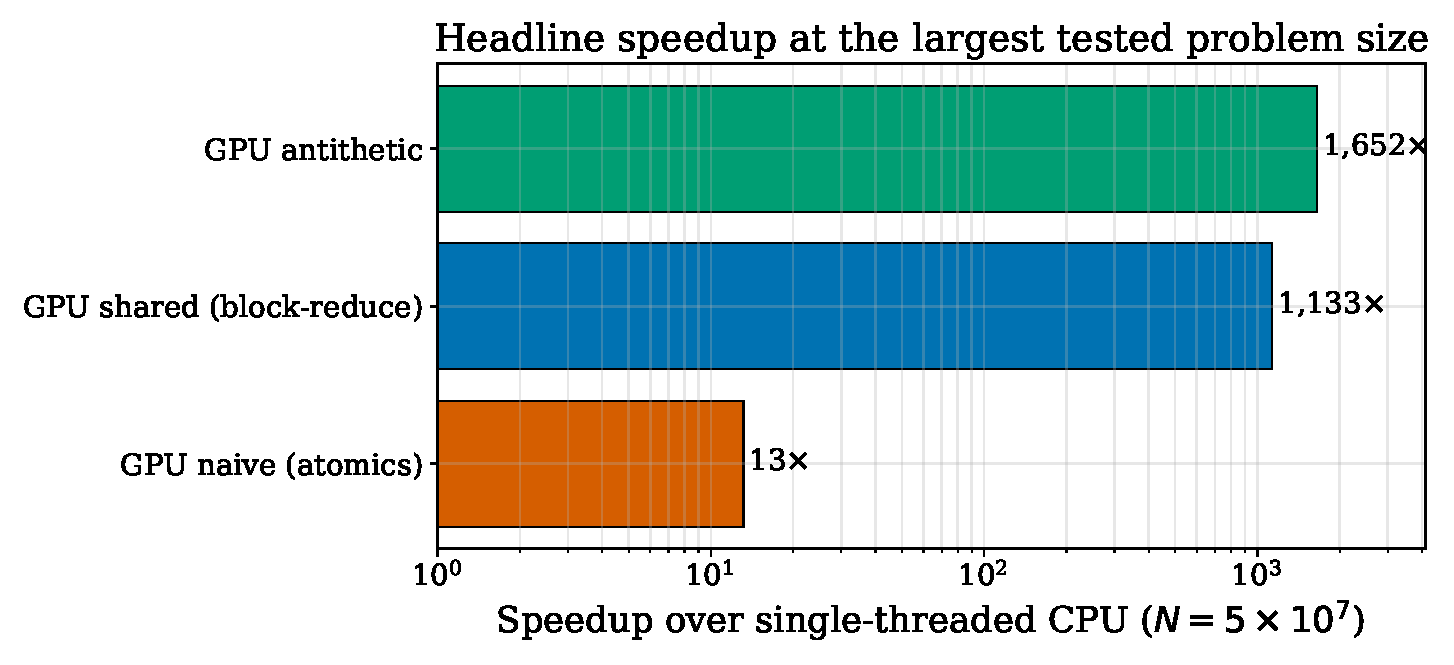
\includegraphics[width=\linewidth]{figures/fig_speedup_bars.pdf}
\end{posterblock}

\begin{posterblock}{C. Profiler-Driven Bottleneck Analysis}
\centering
\begin{tabular}{lrrrl}
\toprule
\textbf{Kernel} & \textbf{Occ.} & \textbf{Compute} & \textbf{DRAM} &
\textbf{Bottleneck}\\
\midrule
\texttt{mc\_naive}      & 93.8\% &  \textbf{2.8\%} & 0.03\% & atomic contention\\
\texttt{mc\_shared}     & 74.6\% & \textbf{79.4\%} & 3.5\%  & compute (arith.-bound)\\
\texttt{mc\_antithetic} & 72.8\% & \textbf{76.4\%} & 5.1\%  & same; statistical win\\
\bottomrule
\end{tabular}\par
\smallskip
\footnotesize Nsight Compute @ $N=10^{7}$, GTX~1650. Occupancy ``looks
healthy'' for \texttt{mc\_naive} but compute throughput exposes the
truth: SMs are full of warps, all stalled on \texttt{atomicAdd}.
\par\medskip
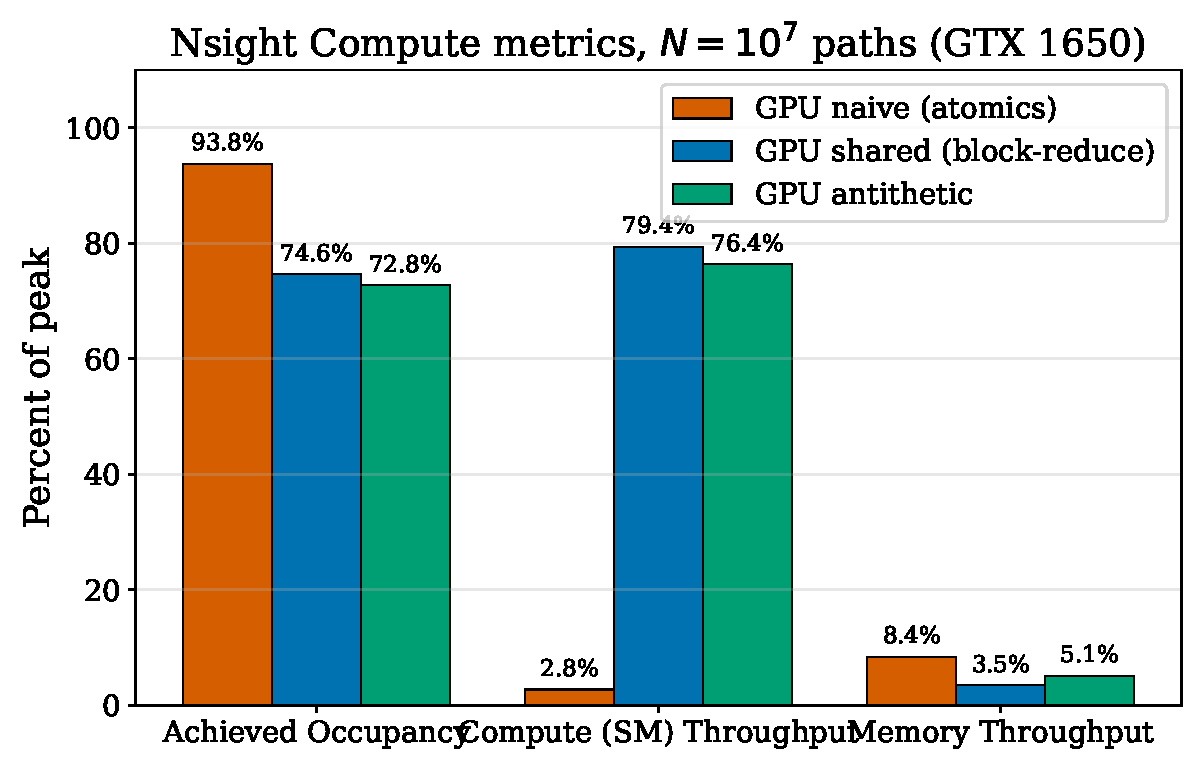
\includegraphics[width=\linewidth]{figures/fig_nsight_metrics.pdf}
\end{posterblock}

\begin{posterblock}{D. Convergence}
\centering
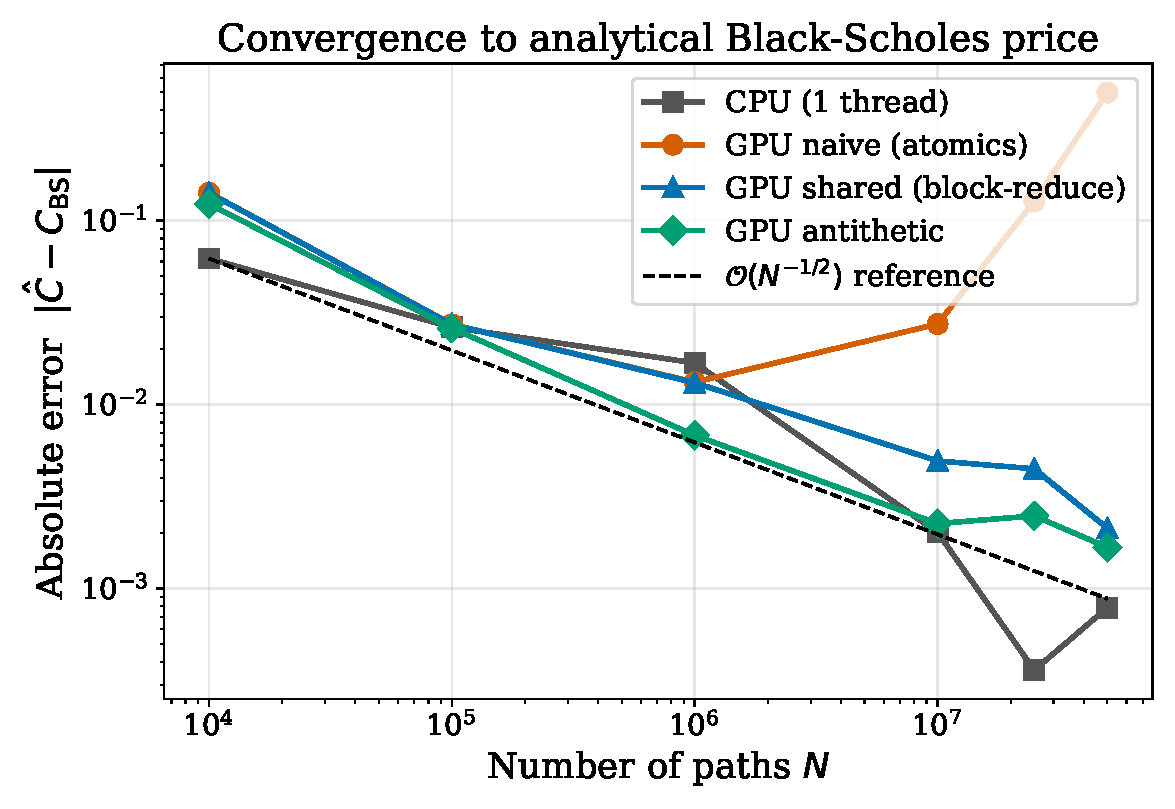
\includegraphics[width=\linewidth]{figures/fig_convergence.pdf}\par
\smallskip
\footnotesize All implementations track the $1/\sqrt{N}$ reference;
antithetic variates sit \textbf{below} the line -- variance reduction
at no additional architectural cost. The naive kernel \emph{leaves}
the line at $N\!\gtrsim\!2.5\!\times\!10^{7}$ because FP32 atomic
accumulation loses precision.
\end{posterblock}

\begin{posterblock}{Conclusion \& Future Work}
\begin{itemize}
\item Block-level reduction with register accumulation
      \textbf{eliminates atomic contention} and lifts achieved
      compute throughput from 2.8\% to 79\%, a
      \textbf{3.7$\times$ kernel-level speedup} over the naive
      version, on top of the GPU-vs-CPU gain.
\item The optimised kernel is then \textbf{arithmetic-bound};
      further wins must attack the RNG (Philox vs XORWOW: smaller
      state, $\sim$3$\times$ faster init).
\item \textbf{Antithetic variates} cut variance by $\sim$50\% on
      monotonic European payoffs at the \emph{same} architectural
      profile -- a statistical, not architectural, speedup.
\item \textbf{FP32 atomic accumulation is unsafe} at scale; this is
      the strongest reason on its own to reduce in shared memory.
\item End-to-end: \textbf{1652$\times$} faster than single-threaded
      CPU at $5\!\times\!10^{7}$ paths, validated to within 0.8\,$\sigma$
      of the Black--Scholes oracle.
\end{itemize}
\textbf{Future work.} XORWOW $\rightarrow$ Philox RNG; CUDA streams
to overlap \texttt{curand\_init} with the pricing kernel; extension
to path-dependent options (Asian, barrier) where MC has no
closed-form competitor.
\end{posterblock}

\begin{posterblock}{References}
\footnotesize
\begin{enumerate}
\item F.~Black and M.~Scholes, ``The Pricing of Options and Corporate
      Liabilities,'' \emph{J. Political Economy}, 1973.
\item P.~Glasserman, \emph{Monte Carlo Methods in Financial
      Engineering}, Springer, 2003.
\item J.~Salmon \emph{et al.}, ``Parallel Random Numbers: As Easy as
      1, 2, 3,'' SC'11.
\item D.~Kirk and W.-m.~Hwu, \emph{Programming Massively Parallel
      Processors}, 4th ed., 2022.
\item NVIDIA cuRAND Library Programming Guide (CUDA 12.4).
\item NVIDIA CUDA C Best Practices Guide.
\item NVIDIA Nsight Compute Documentation.
\end{enumerate}
\end{posterblock}

\end{minipage}

\vspace{8mm}

% =====================================================================
%  Footer
% =====================================================================
\begin{tcolorbox}[enhanced, colback=ituBlue, colframe=ituBlue,
                  arc=2mm, boxrule=0pt, left=10mm, right=10mm,
                  top=3mm, bottom=3mm]
\centering\color{white}\large
Faculty of Computer and Informatics Engineering \quad$\cdot$\quad
Department of Computer Engineering \quad$\cdot$\quad
Istanbul Technical University \quad$\cdot$\quad
İTÜ Ayazağa Campus, 34469, Maslak/Istanbul \quad$\cdot$\quad
\texttt{talhasarlik10@gmail.com}
\end{tcolorbox}

\end{document}
